\documentclass[main]{subfiles}


\title[AutoML: NAS]{Neural Architecture Search}
\subtitle{What is Neural Architecture Search?}
\author[Jovita Lukasik]{Jovita Lukasik}
\date{}

\titlebackground*{images/AutoML_NAS}


%\institute{}
%\date{}

\begin{document}
	
	\maketitle
    
%----------------------------------------------------------------------
%----------------------------------------------------------------------
\begin{frame}{Neural Architecture Design}
\onslide<1-2>
Common Deep Learning procedure for ever-improving neural networks, e.g., on ImageNet~\liturl{Deng et al. 2009}{https://ieeexplore.ieee.org/stamp/stamp.jsp?tp=&arnumber=5206848}:
\onslide<2>
\begin{itemize}
    % \item Deep learning with Convolutional Neural Networks~\liturl{Krizhevsky et al. 2009}{https://proceedings.neurips.cc/paper_files/paper/2012/file/c399862d3b9d6b76c8436e924a68c45b-Paper.pdf} is the main driver for success in computer vision 
    \item Define network topology from \alert{various configuration options} and \alert{various layer types}
\end{itemize}
\onslide<1-2>
\begin{minipage}[t]{0.3\textwidth}    
   \begin{tikzpicture} 
    \node (img6) {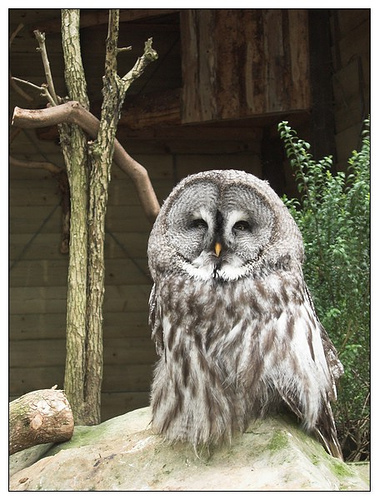
\includegraphics[height=2cm]{images/01/img_net/ILSVRC2012_val_00005770.jpeg}};
    % \node (img5) at (img6.south west) [yshift=0.7cm, xshift=0.2cm] {\includegraphics[height=2cm]{figures/img_net/ILSVRC2012_val_00037220.jpeg}};
   \node (img4) at (img6.south west)  [yshift=0.7cm, xshift=0.5cm] {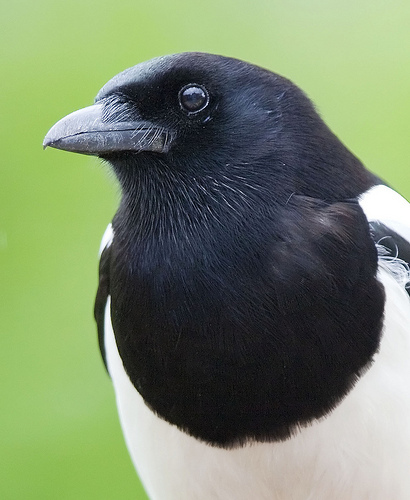
\includegraphics[height=2cm]{images/01/img_net/ILSVRC2012_val_00030073.jpeg}};
   \node (img3) at (img4.south west) [yshift=0.7cm, xshift=0.5cm] {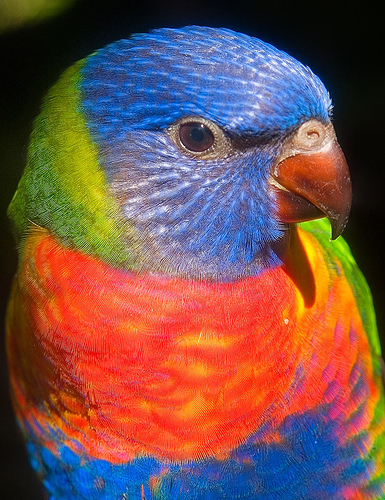
\includegraphics[height=2cm]{images/01/img_net/ILSVRC2012_val_00007778.jpeg}};
    \node (img2) at (img3.south west)  [yshift=0.7cm, xshift=0.5cm] {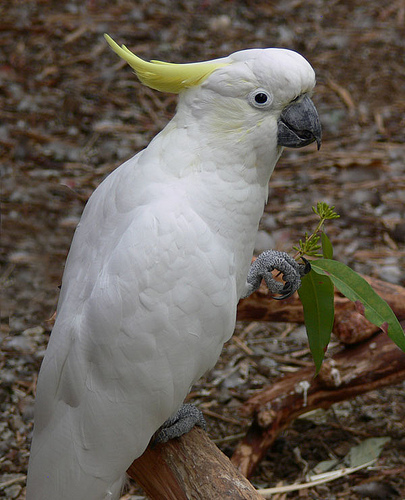
\includegraphics[height=2cm]{images/01/img_net/ILSVRC2012_val_00001288.jpeg}};
   \node (img1) at (img2.south west)  [yshift=0.7cm, xshift=0.5cm] {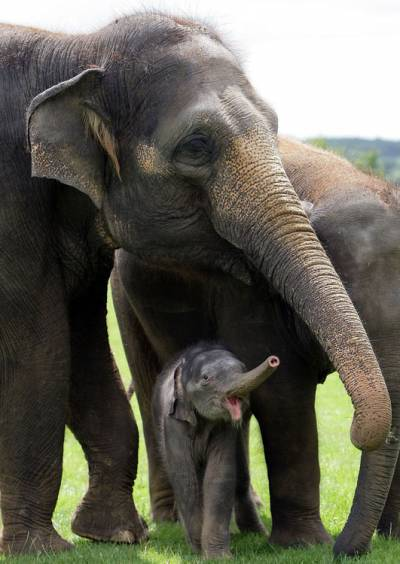
\includegraphics[height=2cm]{images/01/img_net/ILSVRC2012_val_00025237.jpeg}};
   \end{tikzpicture}
      \end{minipage}
      % \vspace{-3cm}
   \hspace{1cm}
   \onslide<2>
   \begin{minipage}{0.1\textwidth}  
   \vspace{-4cm}
      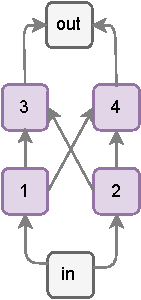
\includegraphics[height=3cm]{images/01/example_graph.pdf}
   \end{minipage}
   \hspace{1.5cm}
\onslide<2>
\begin{minipage}[t]{0.39\textwidth}  
\begin{flushright}
\resizebox{0.8\textwidth}{!}
{ 
% \tikzset{every picture/.style={line width=0.5pt}} %set default line width to 0.75pt        
    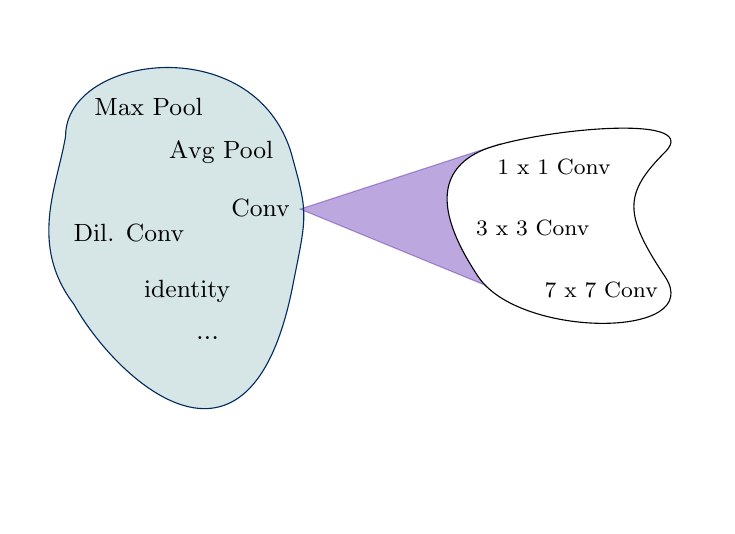
\begin{tikzpicture}[x=0.75pt,y=0.75pt,yscale=-1,xscale=1]
    %uncomment if require: \path (0,300); %set diagram left start at 0, and has height of 300
    
    %Shape: Triangle [id:dp9451139423289833] 
    \draw  [color={rgb, 255:red, 103; green, 58; blue, 183 }  ,draw opacity=0.52 ][fill={rgb, 255:red, 103; green, 58; blue, 183 }  ,fill opacity=0.44 ] (274.46,101.79) -- (370.85,70.38) -- (368.23,140.34) -- cycle ;
    %Shape: Polygon Curved [id:ds8938276343120717] 
    \draw  [fill={rgb, 255:red, 255; green, 255; blue, 255 }  ,fill opacity=1 ] (360.23,74.34) .. controls (380.23,64.34) and (470.23,54.34) .. (450.23,74.34) .. controls (430.23,94.34) and (430.23,104.34) .. (450.23,134.34) .. controls (470.23,164.34) and (380.23,164.34) .. (360.23,134.34) .. controls (340.23,104.34) and (340.23,84.34) .. (360.23,74.34) -- cycle ;
    %Shape: Polygon Curved [id:ds43939369431837927] 
    \draw  [color={rgb, 255:red, 0; green, 41; blue, 92 }  ,draw opacity=1 ][fill={rgb, 255:red, 60; green, 134; blue, 132 }  ,fill opacity=0.21 ] (161.42,66.65) .. controls (161.42,26.65) and (255.42,14.65) .. (271,78) .. controls (278.42,104.65) and (277.42,105.65) .. (271,138) .. controls (250.42,244.65) and (185.42,183.65) .. (165.42,147.65) .. controls (143.42,118.65) and (157.42,90.65) .. (161.42,66.65) -- cycle ;
    
    % Text Node
    \draw (174,47) node [anchor=north west][inner sep=0.75pt]  [font=\small] [align=left] {Max Pool};
    % Text Node
    \draw (210,68) node [anchor=north west][inner sep=0.75pt]  [font=\small] [align=left] {Avg Pool};
    % Text Node
    \draw (240,96) node [anchor=north west][inner sep=0.75pt]  [font=\small] [align=left] {Conv};
    % Text Node
    \draw (164,108) node [anchor=north west][inner sep=0.75pt]  [font=\small] [align=left] {Dil. Conv};
    % Text Node
    \draw (198,135) node [anchor=north west][inner sep=0.75pt]  [font=\small] [align=left] {identity};
    % Text Node
    \draw (368.23,76.34) node [anchor=north west][inner sep=0.75pt]  [font=\footnotesize] [align=left] {1 x 1 Conv};
    % Text Node
    \draw (358,106) node [anchor=north west][inner sep=0.75pt]  [font=\footnotesize] [align=left] { 3 x 3 Conv};
    % Text Node
    \draw (391,136) node [anchor=north west][inner sep=0.75pt]  [font=\footnotesize] [align=left] { 7 x 7 Conv};
    % Text Node
    \draw (223,162) node [anchor=north west][inner sep=0.75pt]   [align=left] {...};
    \end{tikzpicture}
    }
\end{flushright}
\end{minipage}
\end{frame}

\begin{frame}{Limitations of Classical Architecture Design}
\begin{minipage}{0.7\textwidth} 
Overall goal: Find high-scoring and efficient networks \\
Limitations:
\begin{enumerate}
    \item Time-consuming
    \item Trial and error
    \item Expert knowledge
\end{enumerate}
\pause
$\rightsquigarrow$ Complex state-of-the-art architectures are a result of years of trial and error by experts  \\
\end{minipage}
\begin{minipage}{0.25\textwidth} 
\begin{center}
    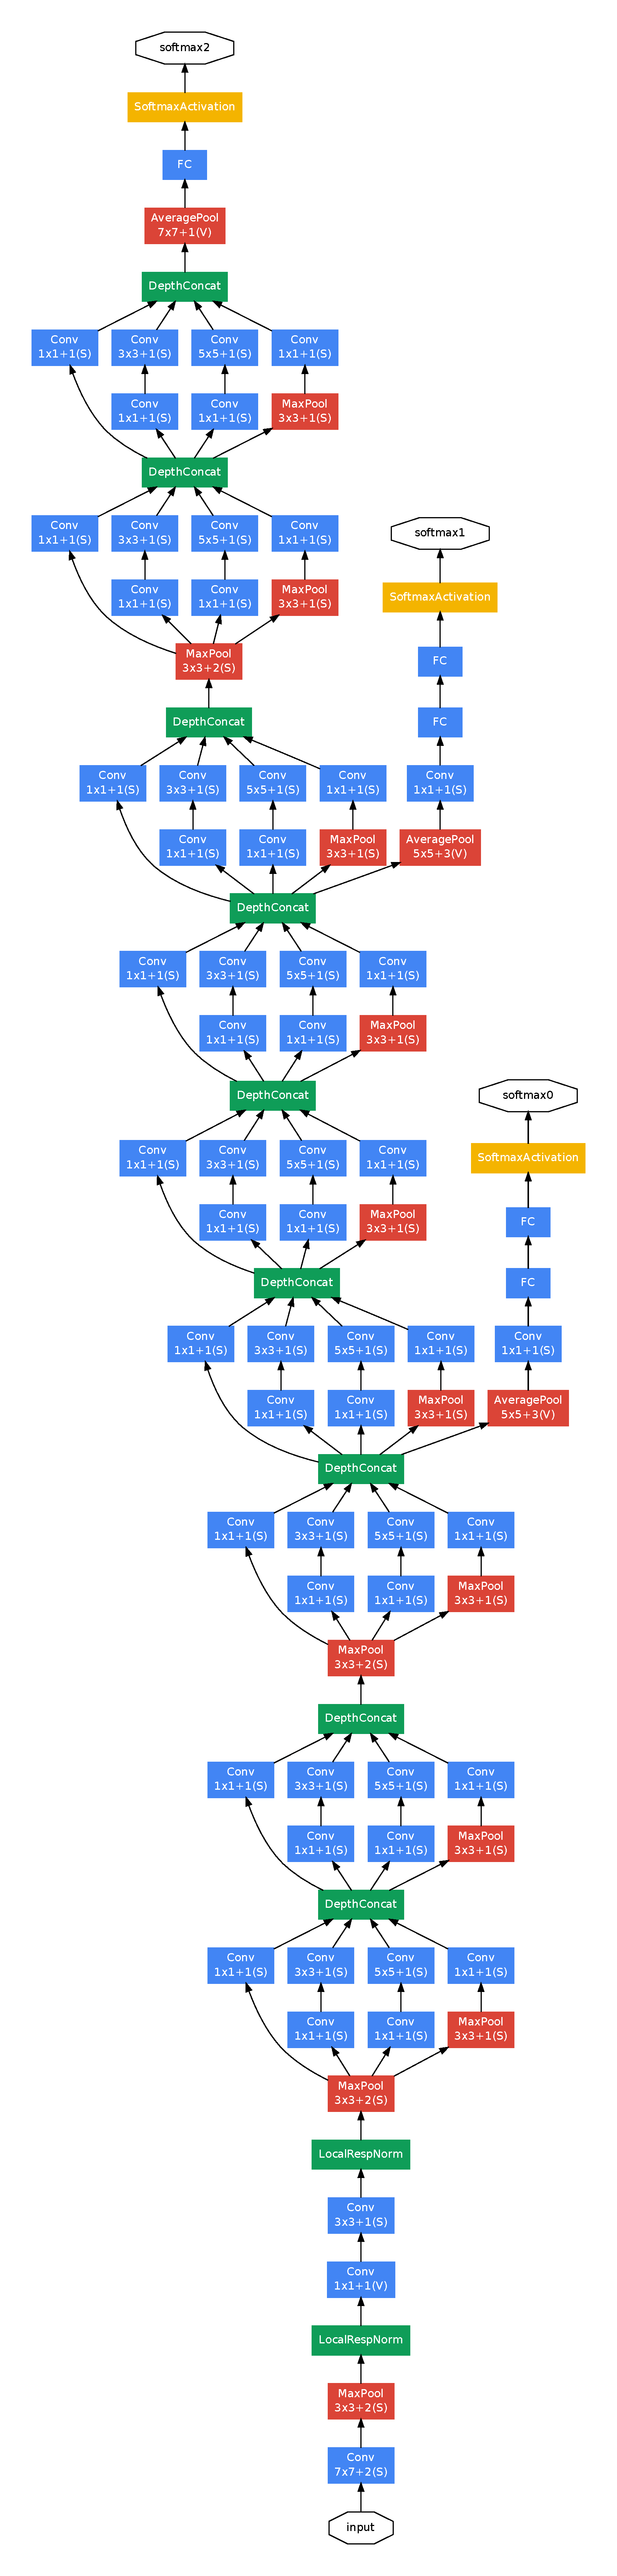
\includegraphics[height=5cm, width=2cm]{images/01/inceptionoverall.pdf}
    \captionof{figure}{GoogLeNet network \liturl{Szegedy et al. 2015}{http://openaccess.thecvf.com/content_cvpr_2015/papers/Szegedy_Going_Deeper_With_2015_CVPR_paper.pdf}}
\end{center}
\end{minipage}
\end{frame}

\begin{frame}{Neural Architecture Search}
\alert{Neural Architecture Search} (NAS): Find a neural network with strong performance in an automatic and efficient way
% \begin{itemize}
    % \item Optionally, subject to a resource constraint 
% \end{itemize}

\begin{minipage}{0.45\textwidth} 
       \begin{itemize}
    \item Overcoming the limitation of the manual design of neural networks 
    \item Intensely researched
    \item Initial methods extremely expensive
    \begin{itemize}
        \item Now more efficient
    \end{itemize}
\end{itemize}
\end{minipage}
\begin{minipage}{0.45\textwidth} 
\begin{center}

\includegraphics[height=4cm]{07_NAS/images/01/no_papers_NAS.png}
    \captionof{figure}{Number of NAS papers by year~\liturl{AutoML.org}{https://www.automl.org/automl/literature-on-neural-architecture-search/?tsr=&yr=0000&type=&auth=&tps_button=Search}}
\end{center}
\end{minipage}
\end{frame}

% \begin{frame}{Neural Architecture Search}
% \begin{minipage}{0.3\textwidth} 
% \begin{itemize}
%     \item NAS models replace human-designed models
% \end{itemize}
% \end{minipage}
% \begin{minipage}{0.65\textwidth} 
% \begin{figure}
%     \centering
%     
\includegraphics[width=0.8\linewidth]{07_NAS/images/01/ErovYVNU0AAyACb.jpeg}
%     \captionof{figure}{NAS designed networks can outperform human designed ones. \liturl{Source}{https://x.com/quocleix/status/1349443438698143744}}
%     \label{fig:placeholder}
% \end{figure}
% \end{minipage}
% \end{frame}

\begin{frame}{Diverse Datasets}
\centering
\begin{table}[]
    \begin{tabular}{l l r}
        CIFAR-100 &  Computer Vision&      
        \begin{minipage}{.2\textwidth}
        
\includegraphics[width=0.15\linewidth]{07_NAS/images/01/cifar100.jpeg}
        \end{minipage}
 \\       
        Spherical & Omnidirectional Vision &       
        \begin{minipage}{.2\textwidth}
        
\includegraphics[width=0.15\linewidth]{07_NAS/images/01/spherical.jpeg}
        \end{minipage} 
        \\
        NinaPro DB5 &  Prosthetics Control &
        \begin{minipage}{.2\textwidth}
        
\includegraphics[width=0.15\linewidth]{07_NAS/images/01/ninapro.jpeg}
        \end{minipage}
        \\
        FSD50K &  Audio Classification &
        \begin{minipage}{.2\textwidth}
        
\includegraphics[width=0.15\linewidth]{07_NAS/images/01/fsd50k.jpeg}
        \end{minipage}
        \\
        Darcy Flow &  PDE Solver &
        \begin{minipage}{.2\textwidth}
        
\includegraphics[width=0.15\linewidth]{07_NAS/images/01/darcy.png}
        \end{minipage}
        \\ 
        PSICOV &  Protein Folding &
        \begin{minipage}{.2\textwidth}
        
\includegraphics[width=0.15\linewidth]{07_NAS/images/01/psicov.jpeg}
        \end{minipage}
        \\
       Cosmic  & Astronomy Imaging & 
       \begin{minipage}{.2\textwidth}
        
\includegraphics[width=0.15\linewidth]{07_NAS/images/01/cosmic.jpeg}
        \end{minipage}
        \\
        ECG  & Medical Diagnostics & 
        \begin{minipage}{.2\textwidth}
        
\includegraphics[width=0.15\linewidth]{07_NAS/images/01/ecg.png}
        \end{minipage}
        \\
        Satellite &  Earth Monitoring &
        \begin{minipage}{.2\textwidth}
        
\includegraphics[width=0.15\linewidth]{07_NAS/images/01/satellite.png}
        \end{minipage}
        \\
    DeepSEA  & Genetic Prediction& 
    \begin{minipage}{.2\textwidth}
        
\includegraphics[width=0.15\linewidth]{07_NAS/images/01/deepsea.png}
        \end{minipage}
        \\
    \end{tabular}
    \caption{NAS-Bench-360~\liturl{Tu et al. 2022}{https://proceedings.neurips.cc/paper_files/paper/2022/file/506630e4a43bb9d64a49f98b9ba934e9-Paper-Datasets_and_Benchmarks.pdf}}
    \label{tab:placeholder}
\end{table}
    
\end{frame}

\begin{comment}
\begin{frame}{Motivation for Future Research}
\begin{minipage}{0.5\textwidth} 
\begin{itemize}
    \item Performance improvements on various tasks due to novel architectures
    \item Can we automate this design process, potentially discovering new components and/or topologies?
\end{itemize}
\end{minipage}
\begin{minipage}{0.4\textwidth} 
\begin{center}
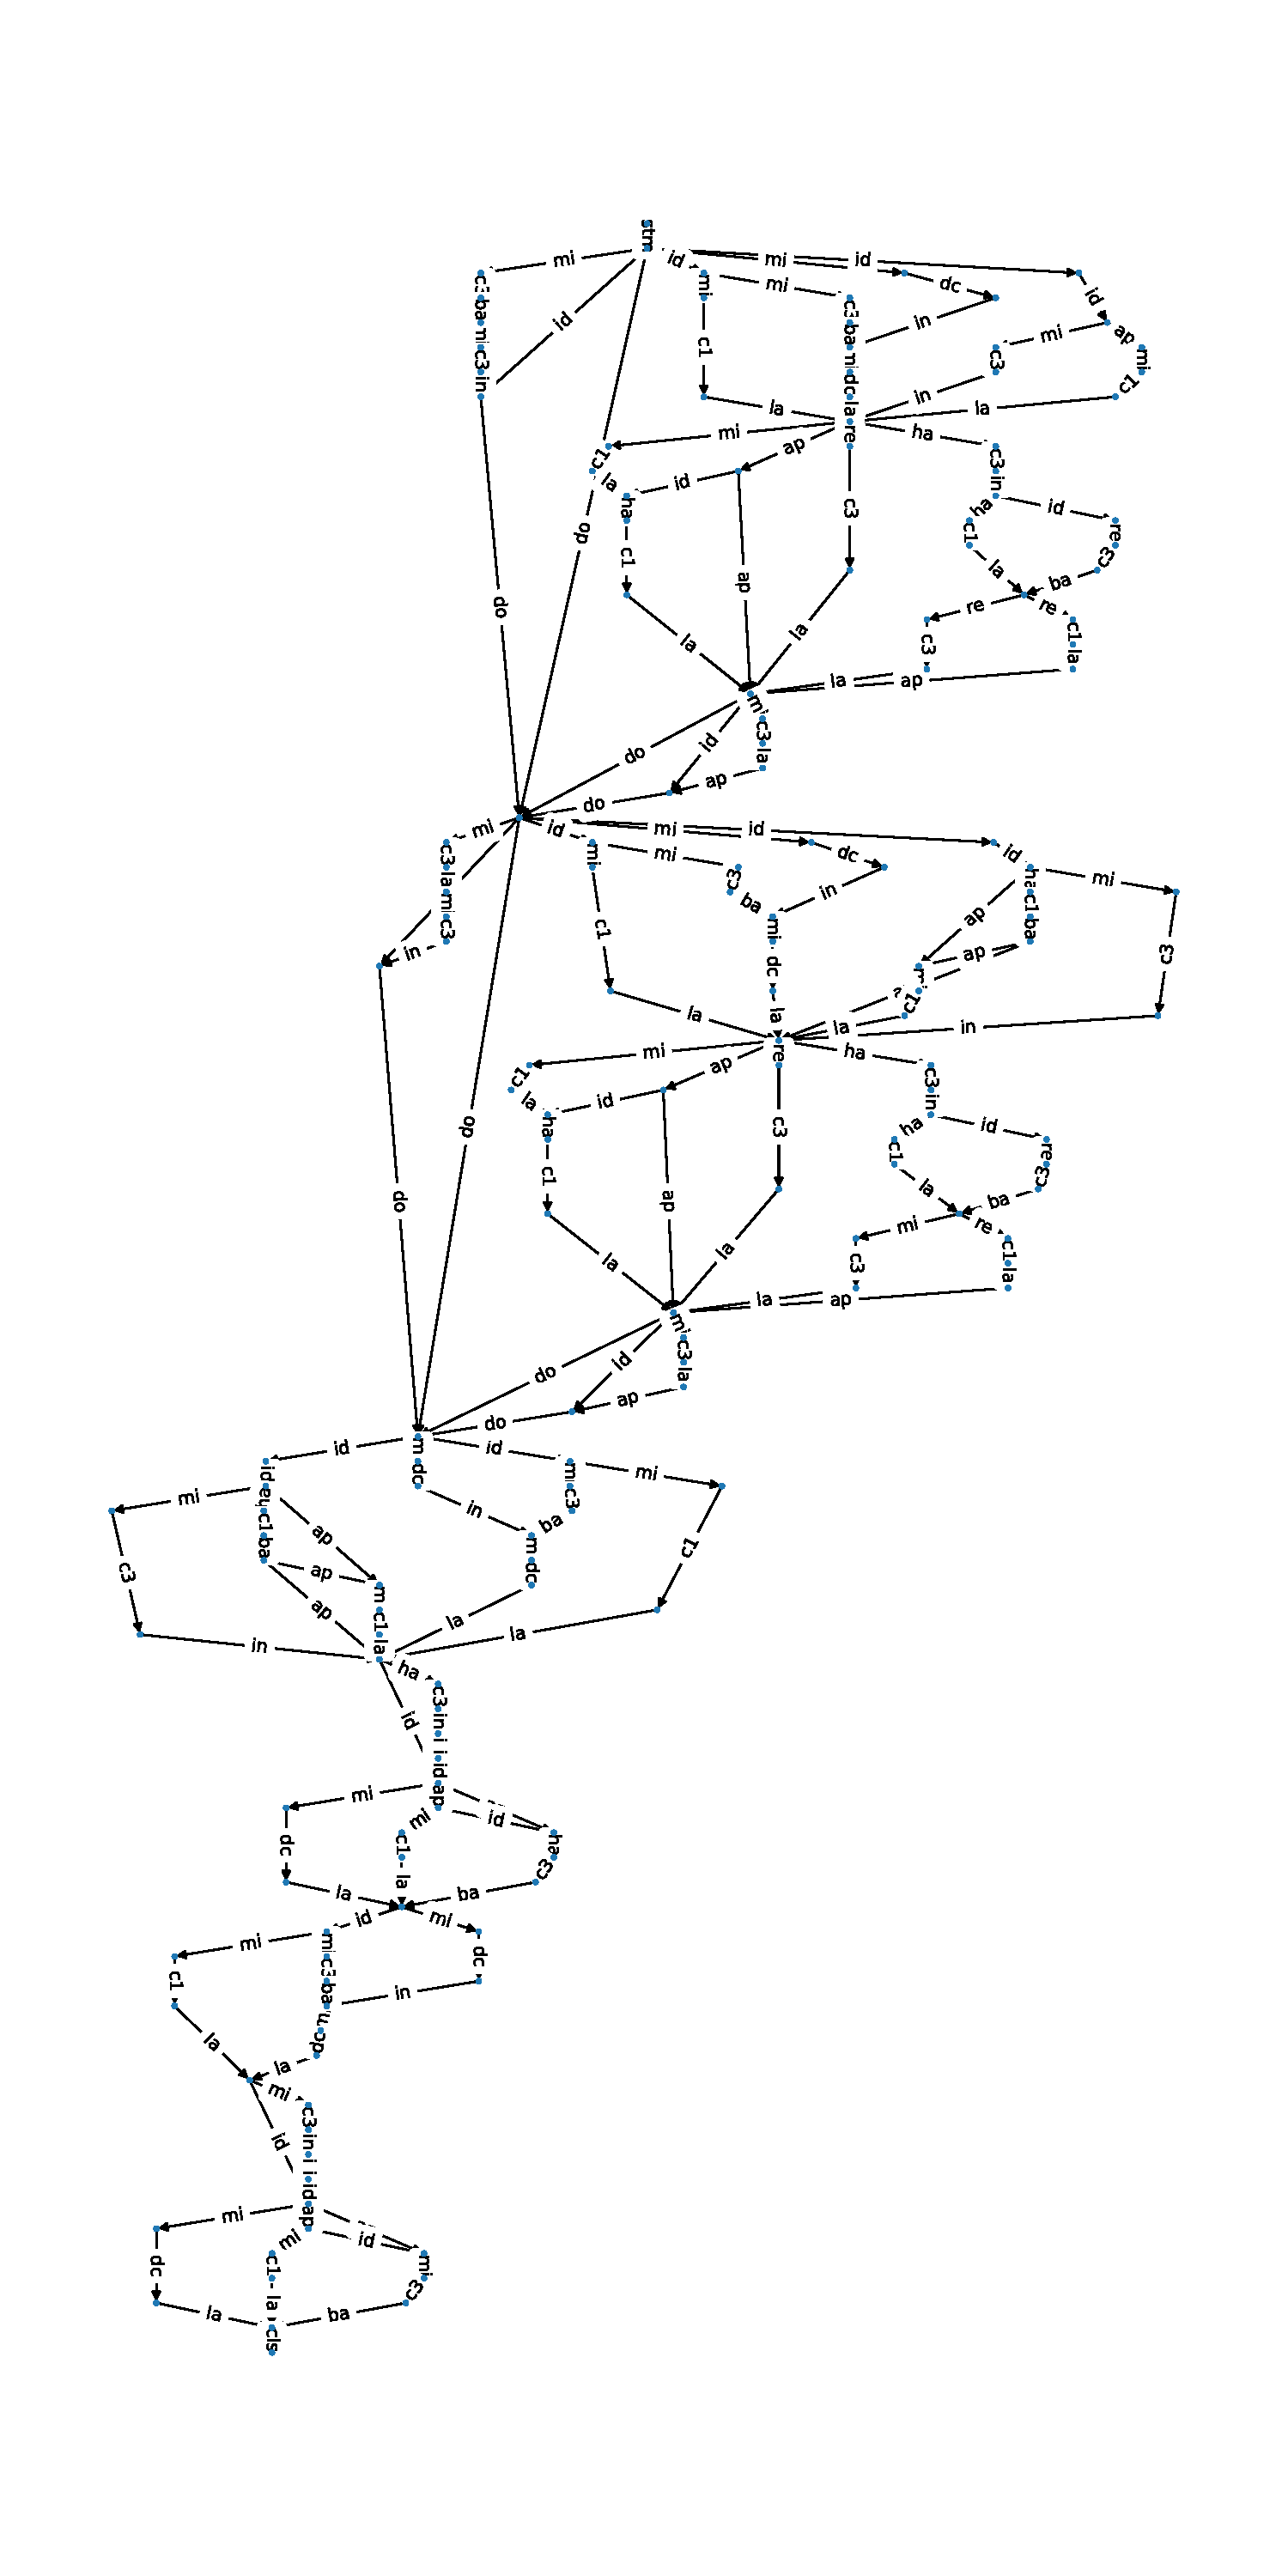
\includegraphics[height=5cm]{images/01/schrodi_cifar10.pdf}
    \captionof{figure}{Best found architecture on the hierarchical search space ~\liturl{Schrodi et al. 2023}{https://openreview.net/pdf?id=Hpt1i5j6wh}}
\end{center}
\end{minipage}
\end{frame}

\begin{frame}{Next Steps with Neural Architecture Search
}
 \begin{itemize}
     \item Early stages of NAS techniques are generally evaluated and developed on benchmarks
     \item How to adapt for other applications?
     \item How to design the search space?
     \item Which method to use?
     \item Do the architecutural design choices scale to larger datasets and architectures?
     \item What is the metric of interest?
     \item Only certain hardware or limited compute available
 \end{itemize}   
\end{frame}
\end{comment}

\begin{frame}{Robustness-Aware NAS}

\begin{columns}
    \begin{column}{0.15\textwidth}
    \centering
     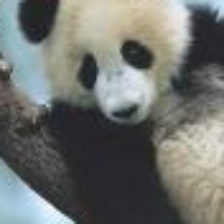
\includegraphics[height=1.5cm]{images/01/panda_577.png} \\
        {panda, \\
        $57.7\%$ confidence}
    \end{column}
    \begin{column}{0.1\textwidth}
    \centering
     \vspace{-1.4cm}
      \[+.007\times~\]
    \end{column}
       \begin{column}{0.15\textwidth}
    \centering
    \vspace{0.9cm}
        
\includegraphics[height=1.5cm]{images/01/nematode_082.png}\\
      FGSM noise
    \end{column}
           \begin{column}{0.05\textwidth}
    \centering
       \vspace{-1.4cm}
       \[=\]
    \end{column}
    \begin{column}{0.15\textwidth}
    \centering
      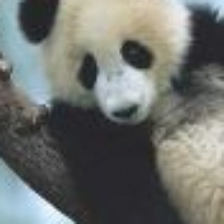
\includegraphics[height=1.5cm]{images/01/gibbon_993.png} \\
        gibbon \\
        $99.3\%$ confidence  
    \end{column}          
\end{columns}
\pause
\vspace{1cm}
    \begin{itemize}
        \item Perturbations on input data can easily cause misclassification~\liturl{Goodfellow et al. 2015}{https://arxiv.org/pdf/1412.6572}
    \end{itemize}
\end{frame}

\begin{frame}{Robustness-Aware NAS}
\begin{columns}
    \begin{column}{0.4\textwidth}
    \begin{itemize}
        \item \textbf{Goal}: find architectures with a good \alert{clean accuracy / robust accuracy} trade-off
    \item \textbf{Challenge}: evaluating robust accuracy requires \alert{adversarial training} (or at minimum adversarial evaluation) — very expensive
    \end{itemize}
    \end{column}          
   
\begin{column}{0.5\textwidth}
    \begin{center}
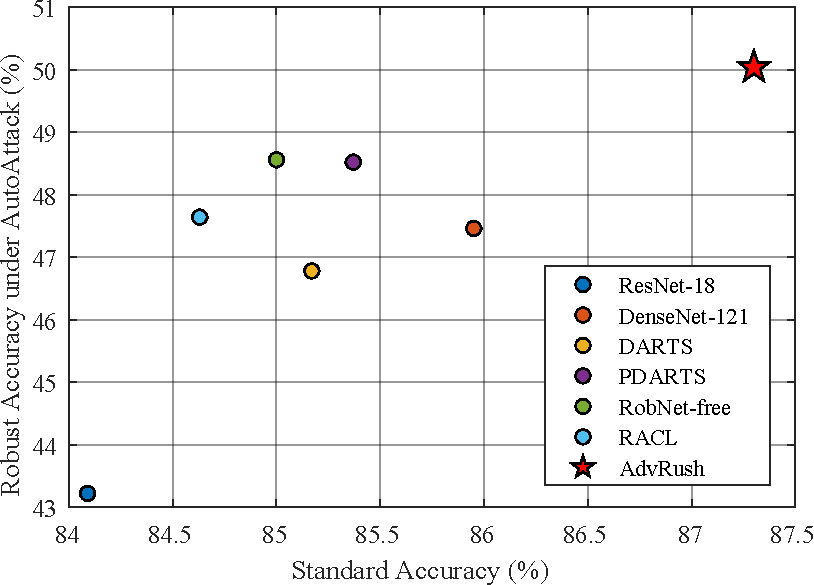
\includegraphics[height=4cm]{images/01/adv_rush_intro_figure.pdf}
    % \captionof{figure}{Standard accuracy vs. robust accuracy evaluation results on CIFAR-10 ~\liturl{Mok et al. 2021}{https://openaccess.thecvf.com/content/ICCV2021/papers/Mok_AdvRush_Searching_for_Adversarially_Robust_Neural_Architectures_ICCV_2021_paper.pdf}}
    \captionof{figure}{\liturl{Mok et al. 2021}{https://openaccess.thecvf.com/content/ICCV2021/papers/Mok_AdvRush_Searching_for_Adversarially_Robust_Neural_Architectures_ICCV_2021_paper.pdf}}
\end{center}
\end{column}
\end{columns}
\end{frame}

\begin{frame}{Hardware-Aware NAS}
\begin{minipage}[c]{0.55\textwidth}
\begin{itemize}
    \item Architectures must run efficiently on \alert{specific hardware targets}: mobile CPUs, embedded FPGAs, data-centre GPUs
    \item The same architecture can have very different latency depending on the hardware
    \item Search for efficient and high-performing architectures automatically
    \pause
    \item[] $\rightsquigarrow$ A single global efficiency metric (e.g.,\ FLOPs) is \textbf{insufficient}; hardware-specific profiling is needed
    \item Often used as a multi-objective setting
\end{itemize}
\end{minipage}
\begin{minipage}[c]{0.4 \textwidth}
    \begin{center}
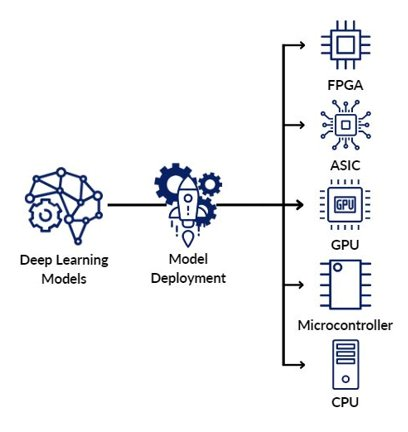
\includegraphics[height=5cm]{images/01/hardware_types.jpg}
    \captionof{figure}{Different hardware types ~\liturl{Benmeziane et al. 2021}{https://arxiv.org/pdf/2101.09336.pdf}}
\end{center}
\end{minipage}
\end{frame}

\begin{frame}{Incorporating Hardware Cost into NAS}
Two main approaches:

\begin{enumerate}
    \item \alert{Constrained search}: add a latency / memory \textbf{constraint} and search for the best accuracy satisfying it
    \begin{itemize}
        \item Direct approach; hard constraints are easy to communicate
        \item Requires re-running the search for each constraint value $\tau$
    \end{itemize}
    \pause
    \item \alert{Multi-objective search (Scalarization)}: combine objectives into a single weighted sum
    \[
        \mathcal{L}(a) = -\cost_{\text{acc}}(a) + \lambda \cdot \cost_{\text{hw}}(a)
    \]
    \begin{itemize}
        \item $\lambda$ controls the trade-off
        \item Changing $\lambda$ moves along the Pareto front — cheap to sweep
        % \item Assumes a linear trade-off which may not hold globally
    \end{itemize}
\end{enumerate}
\end{frame}

\begin{frame}{Beyond Benchmarks: Hardware Efficiency}
%
    \begin{center}
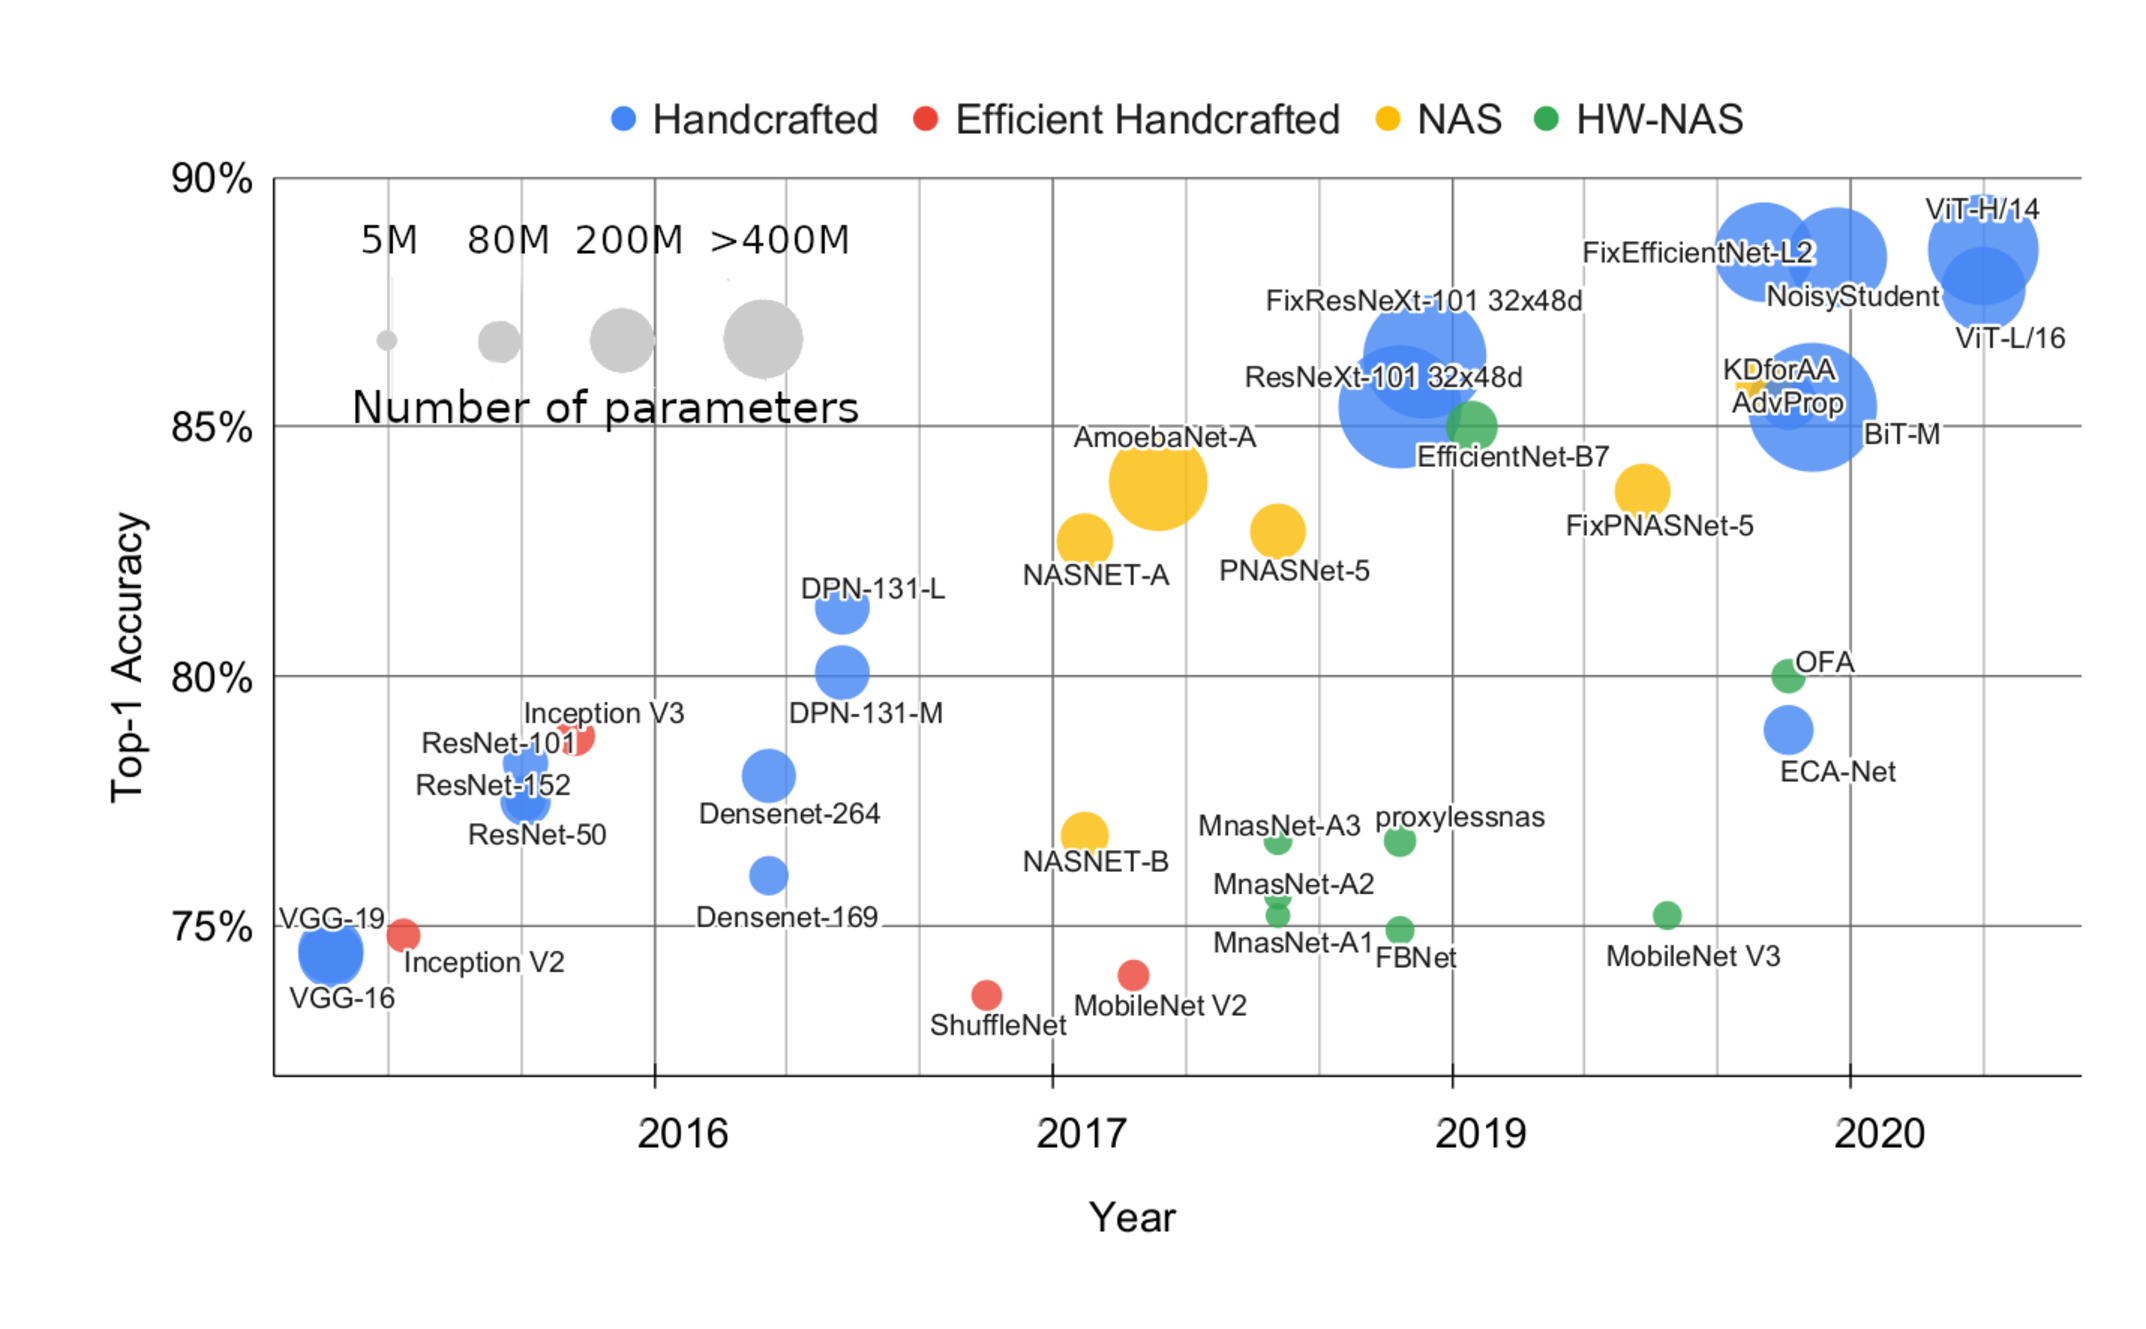
\includegraphics[height=6cm]{images/01/hw_chart.pdf}%
    % \captionof{figure}{Accuracy of various CNN models on ImageNet for image classification with the number of parameters ~\liturl{Benmeziane et al. 2021}{https://arxiv.org/pdf/2101.09336.pdf}}
    \vspace{-1.25em}
    \captionof{figure}{\liturl{Benmeziane et al. 2021}{https://arxiv.org/pdf/2101.09336.pdf}}
\end{center}
\end{frame}

\begin{frame}{Definition of Neural Architecture Search}
\begin{center}
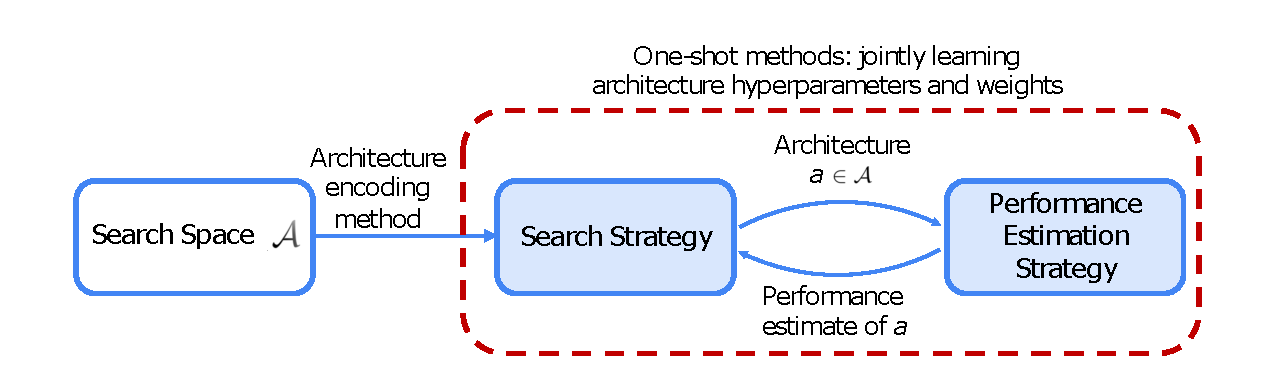
\includegraphics[height=3cm]{images/white_2023_nas_overview.pdf}
\captionof{figure}{Overview of neural architecture search ~\liturl{White et al. 2023}{https://arxiv.org/pdf/2301.08727.pdf}}
\end{center}
\begin{itemize}
    \item Different NAS components
        \begin{enumerate}
            \item Search Space
            \item Search strategy
            \item Performance estimation strategy
        \end{enumerate}
\end{itemize}
% Question: Which component still needs the most human expert knowledge?
\end{frame}
%----------------------------------------------------------------------

\begin{frame}{Summary}
    
Most important insights from this video:

\begin{enumerate}
\item NAS aims to automate the time-consuming process of designing a neural network
\item NAS has shown the ability to perform high on a diverse set of datasets and improve over human designed neural networks
\item  NAS is particularly important for achieving multiple objectives simultaneously, such as dealing with hardware constraints in both constrained and multi-objective search scenarios. 
\end{enumerate}
\end{frame}


\end{document}
